% experiments.tex

\section{Experiments}

\paragraph{Terminology.}
\emph{Cross-attack OOD}: evaluation on attack families unseen during training; benign distribution remains IID throughout (OOD reflects attack-side shift only). $K$: prefix length (number of conversation turns retained). \emph{DAPT}: all Stage-1 adaptations, extending \citet{gururangan2020dontstop} to supervised variants. \emph{Evidence hierarchy} (on synthetic data): vanilla $<$ MLM $<$ classification (Section~\ref{sec:decomposition}).

\subsection{Setup}

\paragraph{Data.}
All synthetic data is generated by Qwen3-8B~\citep{qwen3_2025}.
The IID dataset contains 250 Crescendo~\citep{russinovich2024crescendo} jailbreak and 250 topic-anchored benign conversations, split into training (350), validation (74), and test (76) sets with balanced class ratios (e.g., test = 38 jailbreak + 38 benign).
Stage~1 (DAPT) uses training + validation conversations; Stage~2 (BiGRU) trains on training, early-stops on validation, and evaluates on test.
OOD evaluation pairs attack-specific jailbreak conversations with the 38 IID-test benign conversations: 80 FITD~\citep{fitd2024} (non-discriminative; Section~\ref{sec:decomposition}) + 38 benign = 118 total, 80 Deceptive Delight (DD)~\citep{deceptivedelight2024} + 38 benign = 118 total, and 80 ActorAttack~\citep{ren2024actorattack} + 38 benign = 118 total.
No overlap exists in attack templates across families; benign is IID (same generation pipeline).
A paraphrased version of the IID test set (BERTScore 0.92, lexical overlap 0.20) serves as the adversarial robustness benchmark (Section~\ref{sec:perturbation}).
For human data validation, we use ToxicChat~\citep{lin2023toxicchat} (204 jailbreak + 204 benign from real LMSYS user interactions), entirely independent of Qwen3-8B generation.

\paragraph{Models.}
Seven DeBERTa-v3 variants share the same Stage-2 pipeline and differ only in Stage-1 training (Section~\ref{sec:method}).
Our vanilla DeBERTa+BiGRU configuration is architecturally equivalent to DeepContext~\citep{deepcontext2026}, differing only in encoder choice (DeBERTa-v3-base vs.\ BERT); it serves as our primary baseline.
For cross-encoder validation, we replicate vanilla, MLM, and 9-class variants on RoBERTa-base~\citep{liu2019roberta} (Section~\ref{sec:cross_encoder}).
We also compare TF-IDF LR, LLM-as-judge (Appendix~\ref{sec:llm_judge}), and Llama Guard~3~8B~\citep{metallamaguard3_2024} (zero-shot; evaluates last-response safety given conversation context), which detects only 1.8\% of multi-turn jailbreaks (5/278 pooled recall; Table~\ref{tab:evidence_hierarchy}).

\paragraph{Metrics.}
F1 for binary jailbreak detection at prefix $K$=2 and full conversations (full per-$K$ results in Appendix~\ref{sec:full_prefix}).
OOD results report 3-seed mean$\pm$std (seeds 42, 123, 456) for all variants.
For key pairwise comparisons, we report BCa bootstrap 95\% confidence intervals (10,000 resamples over individual predictions pooled across 3 seeds; this assumes cross-seed independence and is exploratory) and paired permutation tests (10,000 permutations). Seed-level F1 values (Table~\ref{tab:seed_level}, Appendix~\ref{app:seed_level}) confirm all pairwise conclusions hold at every seed.
All standard deviations are computed over 3 random seeds using the population formula ($n$ divisor); Bessel-corrected estimates ($n{-}1$ divisor) are $\approx$22\% larger but do not alter any significance conclusions.
Stage-1: learning rate $2 \times 10^{-5}$, batch 16, 4 epochs, MLM masking 15\%.
Stage-2: two-layer MLP, 20 epochs.

%----------------------------------------------------------------------
\subsection{Cross-Attack Generalization}

\begin{table}[t]
\centering
\small
\caption{Cross-attack generalization (F1) at $K$=2 and full conversation length. IID: Crescendo; OOD: Deceptive Delight (DD). 3-seed mean$\pm$std where noted; full per-$K$ in Appendix~\ref{sec:full_prefix}.}
\label{tab:main_results}
\begin{tabular}{@{}lcc|cc@{}}
\toprule
& \multicolumn{2}{c|}{\textit{IID (Cresc.)}} & \multicolumn{2}{c}{\textit{OOD (DD)}} \\
\textbf{Method} & $K$=2 & Full & $K$=2 & Full \\
\midrule
9-class & \textbf{1.000$\pm$.000} & \textbf{1.000$\pm$.000} & .981$\pm$.013 & \textbf{.994$\pm$.005} \\
MLM-only$^{\ddagger}$ & .974 & 1.000 & \textbf{.993$\pm$.009} & .914$\pm$.115 \\
Vanilla & .978$\pm$.016 & 1.000$\pm$.000 & .479$\pm$.038 & .312$\pm$.026 \\
TF-IDF LR$^{\S}$ & 1.000 & 1.000 & 1.000 & .961 \\
\bottomrule
\end{tabular}
\vspace{-2pt}
{\footnotesize $^{\ddagger}$MLM-only IID reports single seed (42); OOD reports 3-seed. $^{\S}$TF-IDF is deterministic (no std).}
\end{table}

Vanilla encoders collapse under cross-attack transfer; domain-adapted variants recover near-perfect detection (Table~\ref{tab:main_results}, Figure~\ref{fig:cross_attack_bar}).
DD exhibits high lexical separability (TF-IDF F1\,=\,0.961); ActorAttack, where TF-IDF collapses to 0.261, serves as the primary stress test for beyond-lexical generalization.
On OOD DD, vanilla DeBERTa collapses to F1 = 0.312$\pm$0.026, worsening with more turns (0.628 at $K$=1 to 0.312 at Full), consistent with attack turns occupying ``benign'' embedding regions~\citep{bullwinkel2025repeng}.
MLM achieves mean F1 $\geq$ 0.97 at all prefixes $K \leq 5$ without any classification labels; domain exposure alone is sufficient.
At full conversation length, MLM drops to 0.914$\pm$0.115 (seed 456 recall = 0.64), while the 9-class model maintains 0.994$\pm$0.005.
TF-IDF LR reaches F1 = 0.961 on full DD; DD is fully solvable by lexical features.
On structurally complex ActorAttack, TF-IDF collapses to F1 = 0.261 (precision = 1.0, recall = 0.15), while 9-class maintains 0.972$\pm$0.026: a 71\,pp gap. Lexical methods cannot capture multi-persona role-playing attack structure. This establishes a ``difficulty threshold'' for lexical methods parallel to that of vanilla encoders: both succeed on DD and fail on ActorAttack (Section~\ref{sec:limitations}).
Bootstrap CIs confirm non-overlapping intervals (9-class DD Full [0.943, 1.000] vs.\ vanilla [0.202, 0.341]; all permutation $p < 0.0001$). FITD is non-discriminative (all variants F1\,$\geq$\,0.990; Section~\ref{sec:limitations}).

\begin{figure}[t]
\centering
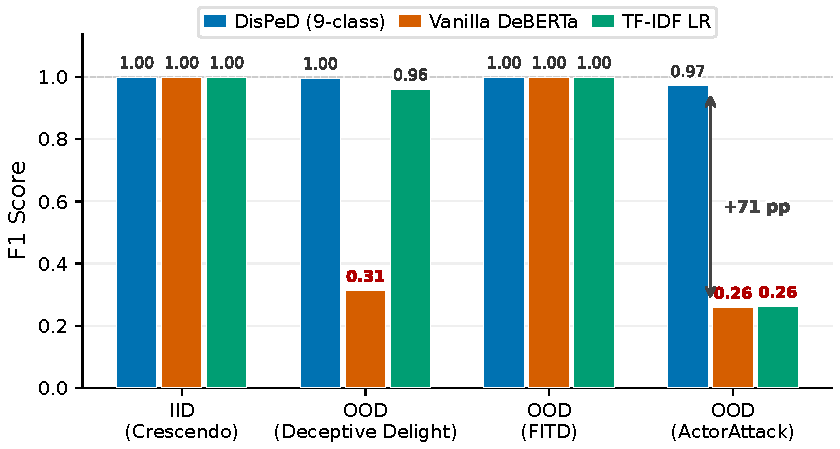
\includegraphics[width=\columnwidth]{figures/paper/fig2_cross_attack_bar.pdf}
\caption{Cross-attack overview (F1 at full conversation length). DisPeD (9-class) maintains near-perfect detection across IID and both OOD families. Vanilla DeBERTa collapses on OOD Deceptive Delight, confirming the necessity of domain-adaptive pretraining. FITD is non-discriminative for all methods (Section~\ref{sec:limitations}).}
\label{fig:cross_attack_bar}
\end{figure}

Prefix-length analysis (Appendix Table~\ref{tab:full_prefix}) shows vanilla F1 drops from 0.628 at $K$=1 to 0.312 at full length. MLM achieves strong early detection ($K$=2: 0.993) but is unstable at full length (0.914$\pm$0.115); the 9-class model maintains 0.972--0.994 across all prefixes. Classification supervision thus stabilizes against distributional drift.

%----------------------------------------------------------------------
\subsection{Decomposing the Detection Mechanism}
\label{sec:decomposition}

\begin{table}[t]
\centering
\small
\caption{Evidence hierarchy on OOD DD and ActorAttack (AA) at full conversation length (3-seed mean$\pm$std where available). Bold indicates best per column. All variants share the same Stage-2 pipeline. Full per-prefix results in Appendix Tables~\ref{tab:full_prefix} and~\ref{tab:actorattack_full}.}
\label{tab:evidence_hierarchy}
\begin{tabular}{@{}lccc@{}}
\toprule
\textbf{Variant} & DD-Full & AA-Full & DD-$K$=2 \\
\midrule
9-class (full model) & .994$\pm$.005 & .972$\pm$.026 & .981$\pm$.013 \\
Binary (2-class) & \textbf{1.000$\pm$.000} & \textbf{.990$\pm$.008} & .994$\pm$.009 \\
Scrambled labels & .994$\pm$.005 & .951$\pm$.043 & .981$\pm$.026 \\
MLM-only$^{\ddagger}$ (no labels) & .914$\pm$.115 & .893$\pm$.080 & .993$\pm$.009 \\
Mean pooling$^{*}$ & .991$\pm$.013 & .962$\pm$.015 & \textbf{1.000} \\
\midrule
Topic classif.\ (5-class) & .541$\pm$.207 & .625$\pm$.141 & .593$\pm$.166 \\
Wikipedia MLM & .904$\pm$.115 & .686$\pm$.297 & .911$\pm$.073 \\
Vanilla DeBERTa & .312$\pm$.026 & .258$\pm$.000 & .479$\pm$.038 \\
TF-IDF LR$^{\dagger}$ & .961 & .261 & \textbf{1.000} \\
Llama Guard~3$^{\P}$ & .025 & .000 & -- \\
\bottomrule
\end{tabular}
\vspace{-2pt}
{\footnotesize $^{*}$9-class encoder with mean pooling replacing BiGRU. $^{\dagger}$Deterministic (no std). $^{\ddagger}$MLM-only IID (Table~\ref{tab:main_results}) is single-seed (42); all OOD values are 3-seed. $^{\P}$Zero-shot; no domain training.}
\end{table}

A clear \emph{evidence hierarchy} emerges across seven variants (Table~\ref{tab:evidence_hierarchy}), ordered by OOD detection at full conversation length on DD:

\vspace{2pt}
\noindent\hspace{0.5em}{\small vanilla (0.312$\pm$0.026) $<$ topic (0.541$\pm$0.207) $\ll$ wiki-MLM (0.904$\pm$0.115) $\approx$ jb-MLM (0.914$\pm$0.115) $<$ scrambled (0.994$\pm$0.005) $=$ 9-class (0.994$\pm$0.005) $\approx$ binary (1.000$\pm$0.000)}
\vspace{2pt}

\paragraph{Domain exposure is the primary mechanism.}
MLM bridges $\sim$60\,pp from vanilla (0.312$\pm$0.026 $\to$ 0.914$\pm$0.115) without labels; this supports the DAPT interpretation~\citep{gururangan2020dontstop}. TF-IDF collapse on ActorAttack (0.261 vs.\ 9-class 0.972) confirms that domain-adapted representations capture features beyond lexical overlap.
All three classification-supervised variants converge to equivalent detection (F1 = 0.994--1.000); McNemar's ($p > 0.13$) and paired permutation tests ($p \geq 0.40$) provide descriptive evidence suggesting equivalence. TOST (margin = 5\,pp) confirms equivalence on DD ($p < 0.01$; Table~\ref{tab:tost_sensitivity}); on ActorAttack, TOST is underpowered (SE\,=\,0.045) despite a 2.1\,pp mean gap. Label quality and granularity are descriptively non-factors for detection.
Classification supervision is associated with 4--20$\times$ lower cross-seed variance over MLM on synthetic OOD (std 0.005 vs.\ 0.115 on DD; observed range across 3 seeds; formal variance ratio tests are not applicable at $n$=3; cross-seed ensemble yields marginal additional gains, Appendix~\ref{app:ensemble}). This stability benefit does not transfer to human-authored data, where classification-supervised variants exhibit the highest variance and pure MLM the lowest (Section~\ref{sec:human_data}).
Appendix~\ref{app:tsne} provides t-SNE visualizations confirming that domain-adapted variants produce tighter, more separable embedding clusters than the vanilla baseline.

\paragraph{Domain specificity is marginal at full length but meaningful for early detection.}
Wikipedia MLM (0.904$\pm$0.115) nearly matches jailbreak-domain MLM at full length (1\,pp gap), though jailbreak-domain text provides an 8\,pp advantage at early prefixes ($K$=2: 0.993 vs.\ 0.911).
Perturbation analysis (Section~\ref{sec:perturbation}) reveals a sharper domain specificity effect: Wikipedia MLM degrades by $\sim$12\,pp under adversarial paraphrasing while jailbreak-domain MLM degrades by only 2.6\,pp.

\paragraph{Misaligned supervision destabilizes generalization.}
Topic classification yields DD-Full F1 = 0.541$\pm$0.207; seed 123 falls \emph{below} vanilla (0.252 vs.\ 0.312). Despite using the same jailbreak-domain training data, topic classification performs worse than Wikipedia MLM (0.904$\pm$0.115), which uses out-of-domain text with no labels. A misaligned objective forces the encoder to allocate capacity to irrelevant features and actively destabilizes representations that MLM would preserve.

\paragraph{Evidence hierarchy on structurally complex attacks.}
ActorAttack~\citep{ren2024actorattack} uses multi-persona steering across longer conversation structures and provides a more challenging OOD benchmark than DD.
The evidence hierarchy at full conversation length is:

\vspace{2pt}
\noindent\hspace{0.5em}{\small TF-IDF (0.261) $\approx$ vanilla (0.258$\pm$0.000) $<$ topic (0.625$\pm$0.141) $<$ wiki-MLM (0.686$\pm$0.297) $<$ jb-MLM (0.893$\pm$0.080) $<$ scrambled (0.951$\pm$0.043) $\approx$ 9-class (0.972$\pm$0.026) $\approx$ binary (0.990$\pm$0.008)}
\vspace{2pt}

TF-IDF collapses from 0.961 (DD) to 0.261 (ActorAttack, precision = 1.0, recall = 0.15). This gap shows that domain-adapted representations capture features beyond bag-of-words.
All classification-supervised variants converge to equivalent performance (0.951--0.990, max gap 3.9\,pp); this extends the DD finding. DAPT provides $\sim$71\,pp over both vanilla (0.258) and TF-IDF (0.261). Full per-prefix results and per-prefix error analysis in Appendix~\ref{sec:actorattack_full} and~\ref{app:aa_error}.

\paragraph{Temporal modeling.}
Mean pooling matches BiGRU on both DD and ActorAttack (F1 gap $\leq$ 1\,pp, overlapping CIs; Appendix~\ref{app:temporal}).
Turn-order shuffling produces negligible change ($|\Delta| < 1$\,pp) across both DeBERTa-v3-base 9-class (DD $\Delta$\,=\,0.000, AA $\Delta$\,=\,$-$0.009, IID $\Delta$\,=\,0.000) and RoBERTa-large 9-class (DD $\Delta$\,=\,+0.001, AA $\Delta$\,=\,$-$0.007, IID $\Delta$\,=\,0.000); detection relies on per-turn representations rather than sequential patterns.

\paragraph{Summary.}
For base-size encoders (125--184M), domain exposure is the primary mechanism; label correctness, granularity, temporal modeling, and domain specificity are non-factors. Classification supervision provides a complementary stability benefit (variance reduced 4--20$\times$) without changing the detection ceiling.
DD and FITD confirm no regression on easier attacks; ActorAttack provides the discriminative evaluation where lexical methods fail.
Detection is stable across conversation lengths (Appendix~\ref{app:length}), near-saturates at 50 conversations (Appendix~\ref{app:data_efficiency}), and is insensitive to auxiliary loss weight (Appendix~\ref{app:lambda}).

%----------------------------------------------------------------------
\subsection{Cross-Encoder Validation}
\label{sec:cross_encoder}

\begin{table}[t]
\centering
\small
\caption{Cross-encoder comparison on OOD Full (3-seed mean$\pm$std). DD = Deceptive Delight, AA = ActorAttack. Bold indicates best per encoder group.}
\label{tab:cross_encoder}
\begin{tabular}{@{}lcc@{}}
\toprule
\textbf{Variant} & DD & AA \\
\midrule
\multicolumn{3}{l}{\textit{DeBERTa-v3-base (184M)}} \\[2pt]
Vanilla & .312$\pm$.026 & .258$\pm$.000 \\
MLM & .914$\pm$.115 & .893$\pm$.080 \\
9-class & \textbf{.994$\pm$.005} & \textbf{.972$\pm$.026} \\
\midrule
\multicolumn{3}{l}{\textit{RoBERTa-base (125M)}} \\[2pt]
Vanilla & .981$\pm$.026 & .466$\pm$.163 \\
MLM & .987$\pm$.018 & .730$\pm$.201 \\
9-class & \textbf{.994$\pm$.005} & \textbf{.939$\pm$.046} \\
\midrule
\multicolumn{3}{l}{\textit{RoBERTa-large (355M)}} \\[2pt]
Vanilla & .927$\pm$.036 & \textbf{1.000$\pm$.000} \\
MLM & .884$\pm$.065 & .874$\pm$.014 \\
9-class & \textbf{.987$\pm$.004} & .946$\pm$.057 \\
\bottomrule
\end{tabular}
\end{table}

To test whether the evidence hierarchy depends on encoder choice, we replicate vanilla, MLM, and 9-class on RoBERTa-base~\citep{liu2019roberta} (Table~\ref{tab:cross_encoder}).
On DD, RoBERTa-base vanilla already achieves 0.981$\pm$0.026 (vs.\ DeBERTa 0.312$\pm$0.026), so DAPT adds only 1.3\,pp. ActorAttack exposes this as DD's simplicity: RoBERTa-base vanilla collapses to 0.466$\pm$0.163, a 51.5\,pp drop, while domain-adapted variants recover (9-class: 0.939$\pm$0.046).

RoBERTa-large (355M) reveals a capacity-DAPT interaction: its effect on ActorAttack reverses (vanilla 1.000 vs.\ 9-class 0.946), while smaller encoders require DAPT to bridge 47--71\,pp. All continued pretraining reduces ActorAttack performance for the largest encoder via representation drift (Table~\ref{tab:roberta_large_lr}), though classification DAPT partially compensates on DD (+6\,pp).

Three encoder scales thus reveal a scale-dependent pattern for the \emph{difficulty threshold}: DeBERTa-v3-base requires adaptation for all attacks, RoBERTa-base only for complex ones, and RoBERTa-large for none (Section~\ref{sec:discussion}).
Classification supervision provides a consistent stability benefit across both base encoders (cross-seed variance: 0.005--0.046 vs.\ 0.026--0.201).
A BERT-base-uncased proxy (110M, matching DeepContext's encoder family) without adaptation achieves DD\,=\,0.318$\pm$0.031 and AA\,=\,0.275$\pm$0.027, comparable to vanilla DeBERTa-v3 (Appendix~\ref{app:bert_proxy}); cross-attack generalization is driven by DAPT rather than encoder architecture.

CKA analysis~\citep{kornblith2019cka} and linear probing confirm that DAPT reshapes representations substantially (Figure~\ref{fig:cka_heatmap}), though comparable CKA shifts yield different detection gains across starting points (Appendix~\ref{sec:cka_heatmap}).

%----------------------------------------------------------------------
\subsection{Mixed-LLM Training}

All preceding experiments use single-source (Qwen3-8B) data. To test whether the evidence hierarchy transfers when training data mixes LLM sources, we train on 250 Qwen + 250 Llama-3.1-8B conversations (Table~\ref{tab:mixed_llm}).
Classification-based DAPT is the only variant that substantially outperforms vanilla: 9-class achieves DD OOD F1\,=\,0.818$\pm$0.096 (+53\,pp over vanilla 0.291$\pm$0.065), while MLM drops to vanilla level (0.289$\pm$0.101). On structurally complex ActorAttack, the advantage narrows (9-class 0.504$\pm$0.107 vs.\ vanilla 0.389$\pm$0.073, +11.5\,pp) with high seed variance, suggesting that limited per-source volume (250 per LLM) constrains generalization to complex attacks. DD and FITD thus primarily validate the baseline rather than the method; ActorAttack, where lexical methods collapse (TF-IDF F1\,=\,0.261) and vanilla encoders fail (F1\,$\leq$\,0.389 across conditions), provides the discriminative evaluation axis.
Mixed-LLM training confirms that classification supervision generalizes across LLM sources where unsupervised pretraining does not; full results in Appendix~\ref{app:mixed_llm}.

%----------------------------------------------------------------------
\subsection{Human Data Validation}
\label{sec:human_data}

Since both training and OOD evaluation data are Qwen3-8B-generated, we validate on ToxicChat~\citep{lin2023toxicchat} (204 human-written jailbreak attempts + 204 benign conversations from real LMSYS interactions).

\begin{table}[t]
\centering
\small
\caption{Human data validation on ToxicChat~\citep{lin2023toxicchat} (macro F1, 3-seed mean$\pm$std). Bold indicates best. Single-turn data from real LMSYS user interactions, independent of Qwen3-8B.}
\label{tab:human_data}
\begin{tabular}{@{}lc@{}}
\toprule
\textbf{Variant} & Macro F1 \\
\midrule
JB-MLM & \textbf{.837$\pm$.013} \\
Wiki-MLM & .791$\pm$.093 \\
Binary & .705$\pm$.072 \\
Scrambled & .616$\pm$.056 \\
9-class & .596$\pm$.087 \\
Topic & .496$\pm$.042 \\
\midrule
Vanilla & .413$\pm$.021 \\
\bottomrule
\end{tabular}
\end{table}

All DAPT variants exceed vanilla by 18--42\,pp (Table~\ref{tab:human_data}): the adapted-vs.-vanilla gap is not a Qwen3-8B generation artifact, and domain exposure on synthetic jailbreak text transfers to human-written attacks.

The ordering reverses: JB-MLM leads (0.837$\pm$0.013) while 9-class ranks lower (0.596$\pm$0.087; $p < 0.001$, non-overlapping CIs). ToxicChat is single-turn, so the classification head provides no advantage; validating the multi-turn hierarchy requires multi-turn human data.

%----------------------------------------------------------------------
\subsection{Perturbation Analysis}
\label{sec:perturbation}

Under adversarial paraphrasing (BERTScore 0.92), classification-supervised variants achieve zero degradation on IID and OOD DD (Table~\ref{tab:ood_perturbation}) while non-adapted models degrade by $\sim$12\,pp ($p < 0.001$); on ActorAttack, DAPT variants degrade ($\Delta$\,=\,$-$20.4\,pp) but maintain 52\,pp over vanilla (Appendix~\ref{sec:perturbation_full}).

%----------------------------------------------------------------------
\subsection{Strategy Trajectory Analysis}
\label{sec:strategy}

The 9-class taxonomy provides interpretable characterization of known attacks ($\kappa$=0.78, $n$=50; Appendix~\ref{sec:strategy_full}) but degrades to near-random on OOD ($\kappa$=0.126; Appendix~\ref{app:strategy_pred}). Its value is twofold: as ablation infrastructure (scrambled labels produce equivalent detection) and as an interpretability tool for known attacks; detection operates through domain-adapted \texttt{[CLS]} embeddings, not strategy accuracy.

%----------------------------------------------------------------------
\subsection{Benign Distribution Shift}
\label{sec:benign_shift}

All preceding OOD results use IID benign data. On WildChat benign conversations, 9-class FPR rises to 68.1\%; cross-LLM error decomposition confirms false positives on unfamiliar benign text drive the collapse (Appendix~\ref{app:wildchat_fpr},~\ref{app:cross_llm}).
